\subsubsection{CMSIS / DSP}
\label{sec:CMSISDSP}

Der Hersteller der ARM Architektur stellt ebenfalls eine leistungsfähige DSP Library für ARM Coretx CPUs bereit.
Diese CMSIS/DSP Library ist bereits als Package über Keil verfügbar.
Anschliessend muss im uVision unter \texttt{Project > Manage Run-Time Environment} die DSP Library angewählt werden \cite{enable-cmsis-dsp-lib}.
Da die Library schon vorkompiliert ist, kann diese entweder als Source oder als Vorkompiliert eingebunden werden.

Die Abbildung \ref{pic:Keil_Cmsis_Symbols} zeigt die Targetoptionen mit den benötigten Werten.

\begin{figure}[H]
	\centering
	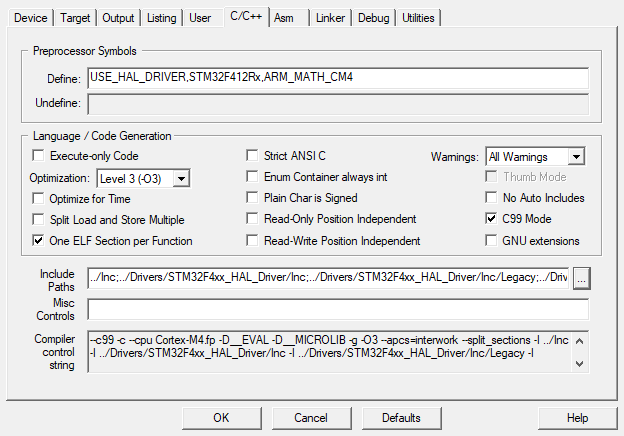
\includegraphics[width=1.0\linewidth]{Keil_Cmsis_Symbols}
	\caption{Options for Target 'P5 DSP Board'}
	\label{pic:Keil_Cmsis_Symbols}
\end{figure}

Des weiteren muss in den Projektoptionen die DSP Library zu den Include Paths hinzugefügt werden.

Unter \texttt{Project > Options for Target 'DSP Board' > C/C++ > Include Paths} muss der String \texttt{../Drivers/CMSIS/DSP/Include} hinzugefügt werden.

Weiterhin muss der CMSIS/DSP Mitgeteilt werden, welche CPU Architektur verwendet wird. Im Falle des \texttt{STM32F4xx} entspricht dies dem Wert \texttt{ARM\_MATH\_CM4}, der als Preprocessor Symbol im selben Konfigurationsfenster hinzugefügt werden muss.
Unter \texttt{Project > Options for Target 'DSP Board' > C/C++ > Preprocessor Symbols > Define:} muss der oben genannte String angefügt werden.





\todo{SB - Muss erklärt werden, wie dieses Package heruntergeladen wird? evtl. bei installation von Keil}

